



\section{Optimus-3}
In this section, we introduce the framework of Optimus-3, designed to organically integrate System 1 action loops with System 2 reasoning capabilities. First, we introduce the \textbf{Knowledge-Enhanced Data Generation Pipeline} (Sec. \ref{pipeline}), which synthesizes high-quality System 2 reasoning traces from raw System 1 trajectories. Then, we detail the \textbf{Dual-Router Aligned MoE Architecture} (Sec. \ref{moe}), specifically engineered to reconcile the computational conflicts between fast, reflexive actions and slow, deliberative reasoning. Subsequently, in Sec \ref{rl}, we elaborate on the \textbf{Multimodal Reasoning-Augmented RL}, a training paradigm designed to activate the agent's System 2 capabilities. Finally, Sec \ref{training_strategy} outlines our multi-stage training strategy.



\subsection{Knowledge-Enhanced Data Generation Pipeline}
\label{pipeline}
\begin{figure*}[htbp]
    \centering
    
\includegraphics[width=0.92\textwidth]{figures/fig5.pdf}
    \caption{Data visualization and statistics of the OptimusM$^4$ dataset. Top: Representative samples across the Planning, Captioning, Embodied QA, Grounding, Reflection, and Action tasks. Bottom: Statistical overview, detailing sample counts, biome distribution, and tech-level distribution for Action data.}
    \label{fig:fig5}
    
\end{figure*}
Currently, while raw gameplay data (System 1 action trajectories) is abundant, datasets capturing the System 2 reasoning traces are scarce. Relying on general-purpose MLLMs for automated annotation often fails, as they lack the domain-specific knowledge of Minecraft, leading to unfeasible plans or hallucinated responses. For instance, most of generic MLLMs \cite{gpt4,lu2024deepseek,dong2024internlm,team2024gemini} lack an understanding of Minecraft crafting recipes (object synthesis relationships), rendering them incapable of generating feasible plans. Furthermore, these models frequently exhibit hallucinations \cite{bai2024hallucination} in vision-centric tasks, such as dense captioning, Embodied Question Answering (EQA), and visual grounding. To address this, we propose a knowledge-enhanced automated data generation pipeline. It injects external knowledge (e.g., domain knowledge graphs, expert models, environmental feedback) as ground-truth constraints to guide and verify the generation process.


As depicted in Figure \ref{fig:fig4}, we first construct a task pool by collecting general items from Minecraft Wiki. For each rollout, we utilize a domain knowledge graph \cite{li2024optimus} to enforce the topological correctness of crafting paths, ensuring the generated plan is feasible. We then employ an expert policy \cite{lifshitz2024steve} to sequentially execute the planned sub-goals. Trajectories verified as successful via environmental feedback signals are archived as action data (observation-action pairs). During execution, visual frames are sampled at a fixed frequency. Subsequently, we utilize environmental feedback (including agent state, inventory, and surrounding objects) as ground-truth for GPT-4o \cite{gpt4} to generate detailed captions. These captions serve as the thinking process for System 2 tasks, enabling the agent to reason based on  visual observations. The annotation process of System 2 tasks is as follows:
\begin{itemize}
    \item \textbf{Embodied QA:} We employ DeepSeek-VL2 \cite{lu2024deepseek} to generate question-answer pairs derived from the generated captions, ensuring captions and QA pairs are factually aligned with the environment feedback.
    \item \textbf{Visual Grounding:} We incorporate Grounding DINO \cite{liu2023grounding} as a vision expert to annotate objects, providing precise bounding boxes that general MLLMs often miss.
    \item \textbf{Reflection:} We employ GPT-4o \cite{gpt4} to annotate execution status based on environment feedback, creating traces of self-correction.
\end{itemize}
We utilize these knowledge sources to filter out hallucinations, and construct Multi-Modal Multi-task Minecraft dataset \textbf{OptimusM$^4$}. It provides the high-fidelity System 2 supervision required to bootstrap the agent's reasoning capabilities. Data visualizations and detailed statistics are presented in Figure \ref{fig:fig5}.



\subsection{Dual-Router Aligned MoE Architecture}
\label{moe}
Unified modeling of System 1 and System 2 introduces a fundamental architectural dilemma: these two modes impose distinct computational requirements. System 1 (Action) demands high-frequency, latency-sensitive processing of local contexts, whereas System 2 (Planning, Reflection) requires deep, computation-intensive reasoning over long horizons. Standard dense architectures enforce a uniform depth, making them either too slow for real-time control or too shallow for complex reasoning. Furthermore, co-training these heterogeneous tasks often leads to gradient interference and negative transfer \cite{moesurvey,huang2025modes}. To resolve these conflicts, we propose the \textbf{Dual-Router Aligned MoE}, a task-aware architecture that structurally enforces System 1/2 coupling through a two-dimensional routing mechanism (Figure \ref{fig:fig2}). 



\subsubsection{Horizontal Routing: Orthogonal Parameter Decoupling}
To prevent gradient interference between conflicting tasks (e.g., visual grounding vs. action prediction), we employ a semantic Task Router.  Unlike token-level soft routing which can lead to load imbalance \cite{shen2025mome}, it deterministically directs input tokens to topologically distinct parameter spaces based on the task type $\mathcal{T}$.

For the $l$-th layer, we replace the standard Feed-Forward Network (FFN) with a hybrid expert module comprising a Shared Knowledge Expert $E_\text{S}$ and Task-Specific Experts $E_\mathcal{T}$. The output hidden state $\mathbf{h}^l$ is computed as:
\begin{equation}
\label{eq:horizontal_routing}
\mathbf{h}^l = \mathbf{x}^l  \oplus (\underbrace{E_{\text{S}}(\mathbf{x}^l)}_{\text{General Knowledge}} + \underbrace{E_{\mathcal{T}}(\mathbf{x}^l)}_{\text{Task-Specific}}),
\end{equation}
where $\mathbf{x}^l$ denotes the input features (after Attention and Normalization). Here, $E_\text{S}$ captures universal semantic patterns across tasks to facilitate positive transfer, while $E_\mathcal{T}$ is exclusively activated for task $\mathcal{T}$. This orthogonal design ensures that the optimization of System 1 control policies is isolated from System 2 reasoning tasks, maintaining a shared representational foundation without task interference.

\subsubsection{Vertical Routing: System-1/2 Adaptive Reasoning}
Complementing the horizontal separation, we introduce a Layer Router to align the model's reasoning depth with the cognitive complexity of the task. Grounded in the Dual-Process Theory \cite{kahneman2011thinking}, this router implements a \textbf{Dynamic Compute Allocation} mechanism. It recognizes that reflexive tasks (System 1) prioritize inference speed, whereas deliberative tasks (System 2) demand reasoning depth.

Formally, we model the vertical routing as a layer selection problem based on task-specific importance. Let $\mathbf{e}_{\mathcal{T}}$ denote the task embedding. We employ a layer router to project the task representation into a layer-wise importance distribution $\boldsymbol{\alpha} \in \mathbb{R}^L$ via a Softmax function:
\begin{equation}
\label{eq:importance_distribution}
\boldsymbol{\alpha} = \operatorname{Softmax}\left( \operatorname{MLP}(\mathbf{e}_{\mathcal{T}}) \right),
\end{equation}
where $\alpha_l$ quantifies the contribution of the $l$-th layer to the current task. To achieve adaptive inference, we introduce a filtering threshold $\tau$ to dynamically determine the set of active layers $\Phi_{\mathcal{T}}$:
\begin{equation}
\Phi_{\mathcal{T}} = \left\{ l \in \{1, \dots, L\} \mid \alpha_l \ge \tau \right\}.
\end{equation}
During the forward pass, layers with importance scores below the threshold are bypassed via residual connections. The state transition is formulated as:
\begin{equation}
\mathbf{x}^{l+1} = \mathbf{x}^l + \mathbb{I}(l \in \Phi_{\mathcal{T}}) \cdot \left( \text{Attn}(\mathbf{x}^l) + \text{MoEBlock}_l(\mathbf{x}^l) \right),
\end{equation}
where $\mathbb{I}(\cdot)$ is the indicator function. This mechanism naturally induces a cognitive dichotomy:
\begin{itemize}
    \item \textbf{System 2 Mode (Deep Path):} For reasoning-intensive tasks (e.g., Planning), the router yields a high-entropy distribution or uniformly high importance across critical reasoning blocks, resulting in $|\Phi_{\mathcal{T}}| \approx L$ to ensure deep reasoning.
    \item \textbf{System 1 Mode (Fast Path):} For interaction-intensive tasks (e.g., Action), the router assigns high probability mass only to a few essential perceptual and control layers. This filters out redundant intermediate computation (i.e., $|\Phi_{\mathcal{T}}| \ll L$), significantly reducing latency.
\end{itemize}
By selectively skipping calculations for non-essential layers, the Dual-Router Aligned MoE achieves a dynamic equilibrium between computational efficiency and reasoning capability, effectively synthesizing the reflexive nature of System 1 and the deliberative depth of System 2 within a unified framework.



\begin{figure*}[htbp]
    \centering
    
\includegraphics[width=0.92\textwidth]{figures/fig6.pdf}
    \caption{Visualization examples of the task-specific fine-grained reward functions in DGRPO. For the Planning task, we design a Dependency-Aware Synthesis Reward, which treats the item's crafting dependency path as thinking reward and assigns fine-grained step-wise supervision as answer reward. For vision-related tasks, we introduce a Hallucination-Aware Consistency Reward that penalizes hallucinated items in the reasoning process and the final answer.
}
    \label{fig:fig6} 
\end{figure*}

\subsection{Dual-Granularity Reasoning-Aware Policy Optimization}
\label{rl}



In the open-ended and dynamic environment of Minecraft, relying solely on Supervised Fine-Tuning (SFT) is insufficient. While Reinforcement Learning (RL) \cite{shao2024deepseekmath} offers a solution to activate reasoning capabilities through exploration \cite{guo2025deepseek}, it lacks fine-grained supervision of the reasoning process. To this end, we propose the \textbf{Dual-Granularity Reasoning-Aware Policy Optimization (DGRPO)} algorithm. It explicitly activates System 2 capabilities by establishing a Process-Outcome Co-Supervision paradigm, utilizing dense rewards to enforce logical consistency between the intermediate reasoning and the final answer.

\subsubsection{Overview of Framework}
DGRPO consists of two progressive phases: a visual-reasoning cold-start phase and a preference alignment phase via reinforcement learning.

\noindent\textbf{Phase 1: Visual-Reasoning Cold Start.}
To initialize the model with basic reasoning capabilities, we perform fine-tuning using Chain-of-Thought (CoT) \cite{wei2022chain} templates. Unlike standard text-only CoT, our approach compels the model to explicitly describe the visual scene within its reasoning trace, thereby grounding high-level reasoning in low-level visual evidence. The objective is defined as:
\begin{equation}
\mathcal{L}_{\text{SFT}} = - \sum_{t=1}^{T} \log \pi_{\theta} \left( y_t \mid x_v, x_{\text{ins}}, y_{<t} \right), \;\;y = [ y^{(\text{think})}; y^{(\text{ans})} ].
\end{equation}
Here, $x_v$ and $x_{\text{ins}}$ denote visual and instructional inputs, respectively. The output $y$ is decomposed into a reasoning process $y^{(\text{think})}$ and a final answer $y^{(\text{ans})}$. This phase serves to mitigate initial hallucinations and activate the model's reasoning capabilities.

\noindent\textbf{Phase 2: Optimization via DGRPO.}
To further robustify the reasoning process, we employ Group Relative Policy Optimization (GRPO) \cite{shao2024deepseekmath} as the optimization backbone. GRPO is particularly advantageous for large-scale MLLMs as it eliminates the need for a separate value function critic. Instead, it utilizes the group average reward as a baseline, reducing computational overhead while stabilizing training.
Formally, given an input $x$, the policy $\pi_{\theta}$ samples a group of $G$ outputs $\{y_1, y_2, \dots, y_G\}$. The optimization objective is formulated as:
\begin{equation}
\begin{split}
\frac{1}{G} \sum_{i=1}^{G} \frac{1}{\left| y_{i} \right|} \sum_{t=1}^{\left| y_{i} \right|}
\Big\{
\min \Big[
  r_{\theta}\left(x, y_{i}\right) A_{i,t},
  \\
  \operatorname{clip}\big( r_{\theta}\left(x, y_{i}\right), 
  1-\varepsilon, 1+\varepsilon \big) A_{i,t}
\Big] - \lambda D_{KL}
\Big\}
\end{split}
\end{equation}

\begin{equation}
r_{\theta }\left ( x, y_{i}  \right ) = \frac{\pi _{\theta } \left ( y_{i,t} \mid x,y_{i,<t}  \right )  }{\pi _{\theta_{old}} \left ( y_{i,t} \mid x,y_{i,<t}  \right ) } , 
\end{equation}

\begin{equation}
D_{KL} = \frac{\pi _{ref } \left ( y_{i,t} \mid x,y_{i,<t}  \right )  }{\pi _{\theta} \left ( y_{i,t} \mid x,y_{i,<t}  \right ) } - \log\frac{\pi _{ref } \left ( y_{i,t} \mid x,y_{i,<t}  \right )  }{\pi _{\theta} \left ( y_{i,t} \mid x,y_{i,<t}  \right ) }  -1,
\end{equation}
where \( A_{i,t} \) denotes the advantage function, \( \varepsilon \) and \( \lambda  \) are hyperparameters, and \( \pi_{\theta_{old}} \) and \( \pi_{ref} \) represent the old policy and the reference model, respectively. 

\subsubsection{Dual-Granularity Dense Reward Design}
Standard GRPO algorithm relies on sparse outcome rewards (e.g., success/failure), which treat the reasoning process as a black box. Crucially, such answer-only supervision fails to penalize flawed reasoning that accidentally yields the correct response (i.e., spurious correlations). DGRPO addresses this by introducing a \textbf{Process-Outcome Co-Supervision} mechanism. We design task-specific dense rewards that provide fine-grained feedback on both the \textit{reasoning process} ($R_{\text{think}}$) and the \textit{final answer} ($R_{\text{ans}}$). As illustrated in Fig. \ref{fig:fig6}, the reward system is tailored for two primary task categories.


\noindent\textbf{Dependency-Aware Synthesis Reward}.
In long-horizon planning tasks, the core challenge is strictly adhering to the hierarchical synthesis logic of Minecraft. We propose the Dependency-Aware Synthesis Reward ($R_{\text{DAS}}$) to enforce topological consistency with the domain knowledge graph.
Let $\mathcal{G}_{\text{syn}}$ be the ground-truth synthesis dependency graph. The total reward $R_{\text{DAS}}$ is a weighted sum of the thinking reward $R_\text{think}$ and plan accuracy reward $R_\text{ans}$:
\begin{equation}
R_{\text{DAS}}(y) = \underbrace{\frac{1}{M} \sum_{m=1}^{M} \mathbb{I}(y^{(\text{think})}_m \in \mathcal{G}_{\text{syn}})}_{R_{\text{think}}} + \underbrace{\frac{1}{N} \sum_{n=1}^{N} \mathbb{I}(y^{(\text{ans})}_n = y^{(\text{gold})}_n)}_{R_{\text{ans}}},
\end{equation}
where $\mathbb{I}(\cdot)$ is the indicator function, and $M$ and $N$ represent the number of reasoning steps and plan steps, respectively. $R_{\text{thinking}}$ encourages the model to explicitly verify material prerequisites in its thought chain, while $R_{\text{answer}}$ ensures the final plan sequence matches the optimal path.


\noindent\textbf{Hallucination-Aware Consistency Reward}.
For tasks requiring precise visual grounding (Embodied QA, Reflection, Grounding), the primary failure mode is perceptual hallucination \cite{bai2024hallucination}. We introduce the Hallucination-Aware Consistency Reward ($R_{\text{HAC}}$) to penalize the generation of non-existent entities during reasoning.
Let $\mathcal{S}_{\text{gold}}$ denote the set of ground-truth objects present in the scene. The reward function is defined as:
\begin{equation}
R_{\text{HAC}}(y) = \underbrace{\frac{1}{N} \sum_{n=1}^{N} \mathbb{I}(y^{(\text{think})}_n \in \mathcal{S}_{\text{gold}})}_{R_{\text{think}}} + \underbrace{r_{\text{task}}(y^{(\text{ans})}, y^{(\text{gold})})}_{R_{\text{ans}}}.
\end{equation}
Here, $R_\text{think}$ explicitly measures perceptual precision (analogous to $1 - \texttt{CHAIR}$ \cite{rohrbach2018object}), forcing the agent to ground its reasoning in visual perception to answer questions.
The answer reward $R_\text{ans}$ adapts to the specific task format:

\begin{itemize}
    \item \textbf{Embodied QA}: We utilize ROUGE-L F1 score to measure the accuracy of the agent's responses.
    \item \textbf{Reflection}: We utilize binary success indicators to measure accuracy of the agent's decisions.
    \item \textbf{Visual Grounding:} We implement a strict \textbf{IoU-Density Reward} to penalize imprecise bounding boxes. Given the Intersection-over-Union (IoU) score $u$ between predicted and ground-truth boxes:
    \begin{equation}
    R_{\text{ans}} = 
    \begin{cases}
    1, & \text{if } u \ge \alpha \\
    \eta u, & \text{if } \beta \le u < \alpha \\
    0, & \text{if } u < \beta
    \end{cases}
    \end{equation}
    Here, $\alpha$ and $\beta$ are hyperparameters in the range $(0, 1)$, and $\eta$ is a weighting coefficient.
\end{itemize}


\begin{figure}[htbp]
\centering
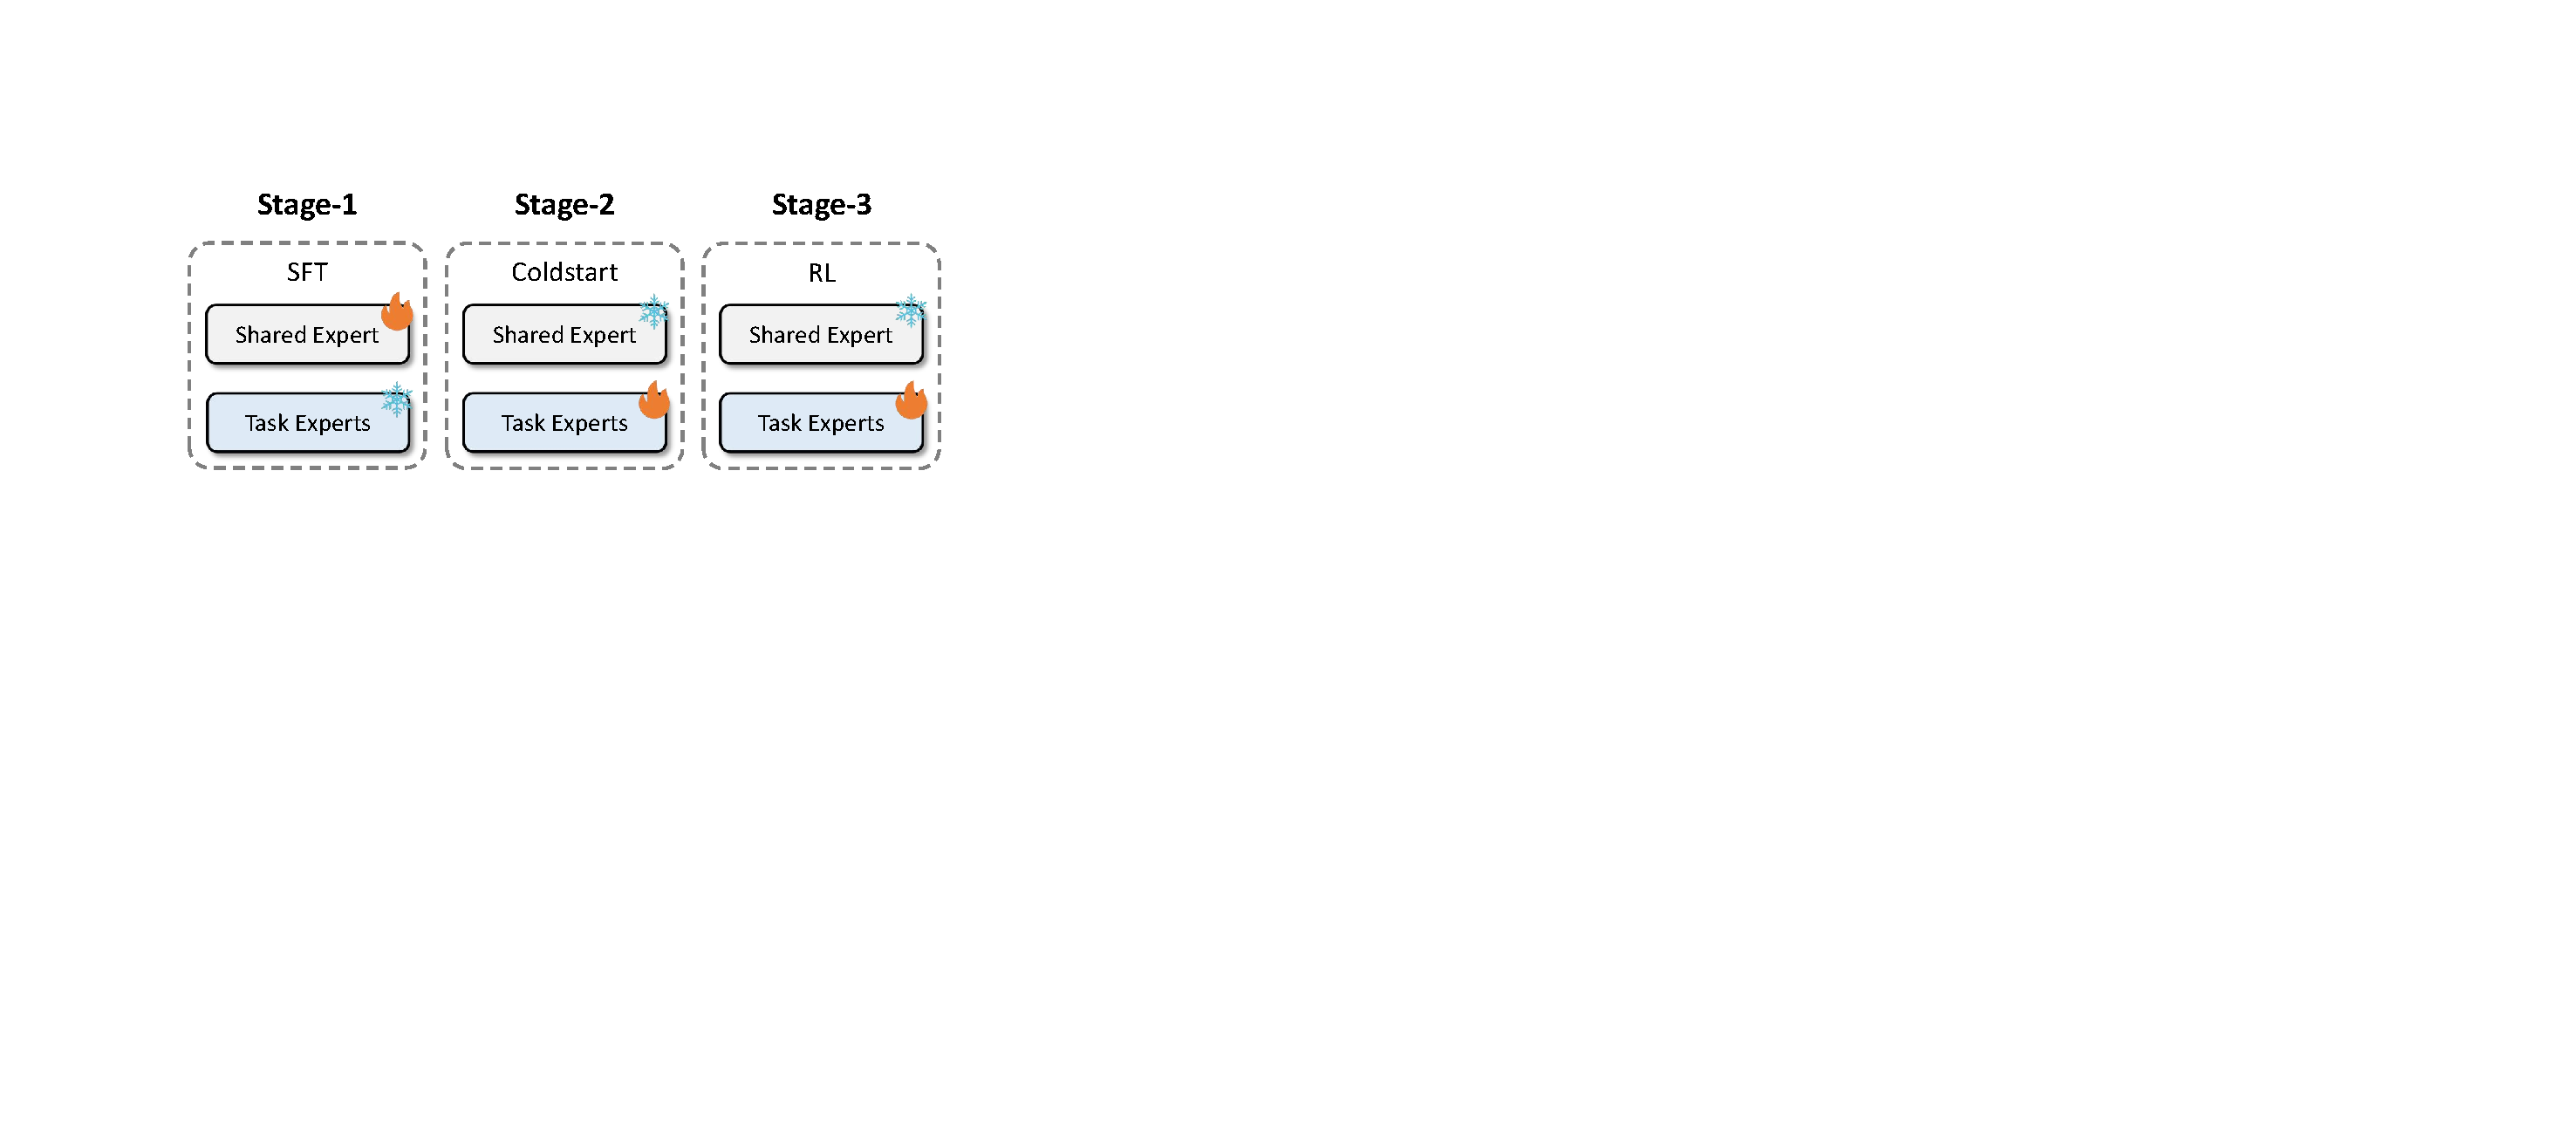
\includegraphics[width=0.45\textwidth]{figures/fig7.pdf}
\caption{The stage-wise training strategy. \textbf{Stage-1}: We train the shared knowledge expert via Supervised Fine-Tuning (SFT). \textbf{Stage-2}: We train the task experts with multimodal reasoning fine-tuning (Coldstart). \textbf{Stage-3}: We further train the task experts with Reinforcement Learning (RL).}
\label{fig:fig7}
\end{figure}
Additionally, we add a Format Reward with weight $\lambda_f$ to each task, requiring the agent's response to follow the format $<\texttt{think}>...</\texttt{think}><\texttt{answer}>...</\texttt{answer}>$.


\subsection{Training Strategy}
\label{training_strategy}
To ensure stable convergence, we adopt a three-stage training strategy (as illustrated in Fig. \ref{fig:fig7}) for Optimus-3.

\noindent\textbf{Stage-1}: In this stage, we initialize the shared knowledge expert from a dense model, then train it via supervised fine-tuning. The shared knowledge expert is trained across all tasks to capture common semantic representations. 

\noindent\textbf{Stage-2}: In this stage, we initialize the task experts from shared expert, then freeze the shared knowledge expert. The task experts are trained via the fine-tuning (coldstart) to activate multimodal reasoning capabilities. While the Action expert is trained via imitation learning \cite{li2025optimus}.

\noindent\textbf{Stage-3}: We refine the System 2 experts (Planning, Perception, Reflection) via the DGRPO algorithm. By optimizing against the proposed dual-granularity rewards, the agent learns to generate reasoning chains that are both logically sound and visually faithful.


